\chapter{DESAIN DAN PERANCANGAN}
    Pada bab ini dibahas mengenai analisis dan perancangan sistem.
	
    \section{Kasus Penggunaan}
    	Dalam sistem ini hanya ada satu aktor yaitu \textit{administrator} jaringan yang akan mengatur penyimpanan konfigurasi. Diagram kasus penggunaan digambarkan pada Gambar \ref{usecase}.
        \begin{figure}[H]
			\centering
			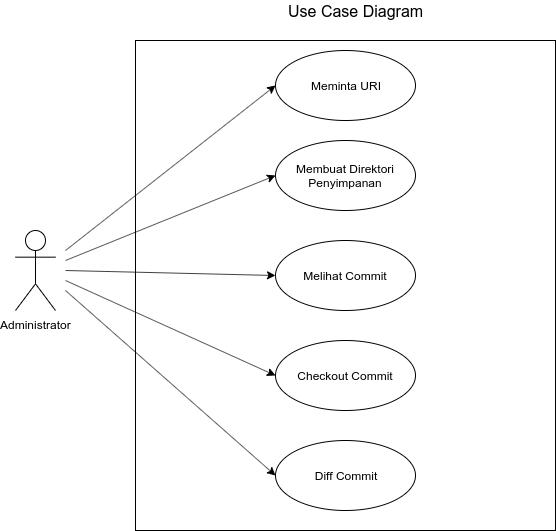
\includegraphics[width=8cm,height=8cm]{Images/C-3/UC.png}
			\caption{Diagram Kasus Penggunaan}
			\label{usecase}
		\end{figure}
        \indent Diagram kasus penggunaan pada Gambar \ref{usecase} dideskripsikan masing-masing pada Tabel \ref {tabelKodeKasusPenggunaan}.
        
        \begin{longtable}{|p{0.25\textwidth}|p{0.24\textwidth}|p{0.35\textwidth}|} % L = Rata kiri untuk setiap kolom, | = garis batas vertikal.
		    	
		    	% Kepala tabel, berulang di setiap halaman
		    
		    	
		    	 \caption{Daftar Kode Kasus Penggunaan} \label{tabelKodeKasusPenggunaan} \\
		    	\hline
		    		\textbf{Kode Kasus Penggunaan} & \textbf{Nama Kasus Penggunaan} & \textbf{Keterangan} \\ \hline
		    	\endfirsthead
		    	\caption[]{Daftar Kode Kasus Penggunaan}   \\
		    	\hline
		    		\textbf{Kode Kasus Penggunaan} & \textbf{Nama Kasus Penggunaan} & \textbf{Keterangan} \\ \hline
		    	\endhead
		    	\endfoot
		    	\endlastfoot
		    	
		    	UC-0001 & Meminta URI. & \textit{Administrator} dapat meminta alamat URI untuk mengirim konfigurasi dari perangkat jaringan.\\ \hline
		    	UC-0002 & Membuat Direktori Penyimpanan.  & \textit{Administrator} dapat membuat direktori untuk menyimpan konfigurasi dari perangkat jaringan.\\ \hline
		    	UC-0003 & Melihat Commit. & \textit{Administrator} dapat melihat riwayat commit dalam repositori perangkat. \\ \hline
		    	UC-0004 & Checkout Commit. & Administrator dapat berpindah commit (checkout) sesuai dengan versi commit yang diinginkan. \\ \hline
		    	
		    \end{longtable}

	\section{Arsitektur Sistem}
		Pada sub-bab ini, dibahas mengenai tahap analisis dan kebutuhan bisnis dan desain dari sistem yang akan dibangun.

		\subsection{Desain Umum Sistem}
			Sistem yang dibuat dalam tugas akhir ini adalah sistem yang dapat mengatur penyimpanan konfigurasi perangkat jaringan. Sistem yang dikembangkan mendukung metode pengiriman konfigurasi TFTP dan FTP. Ketika perangkat jaringan mengirim konfigurasi maka sistem akan secara otomatis melakukan commit pada repositori perangkat jaringan.\\
			\indent Dalam sistem ini akan terdapat thread yang berfungsi untuk mengawasi setiap perubahan yang terjadi pada repositori perangkat jaringan. Setiap ada perubahan pada repositori maka thread langsung melakukan update commit pada repositori.\\
			\indent Sistem ini akan digunakan oleh administrator jaringan yang mana bisa meminta URI repositori, membuat repositori, melihat riwayat commit pada repositori, dan melakukan checkout ke commit yang diinginkan. Penjelasan secara umum arsitektur sistem akan diuraikan pada Gambar \ref{DesainUmumSistem}.\\
                \begin{figure}[H]
                    \centering
                    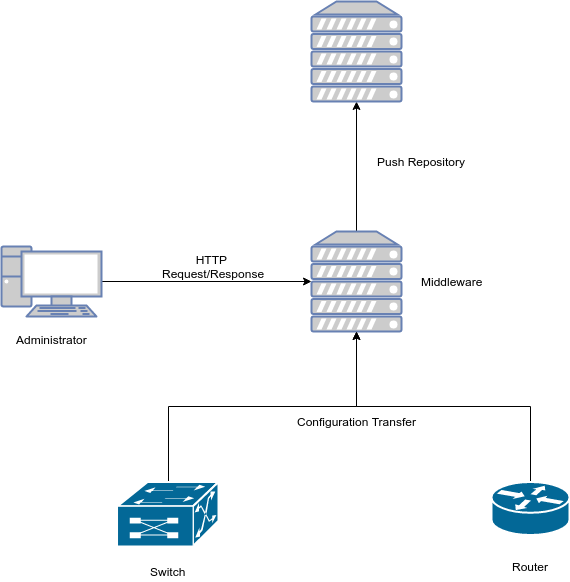
\includegraphics[width=8cm,height=9cm]{Images/C-3/DesainUmumTA.png}
                    \caption{Desain Umum Sistem}
                    \label{DesainUmumSistem}
                \end{figure}
                
		\subsection{Perancangan Repositori Perangkat }
			Repositori perangkat adalah komponen untuk menyimpan file konfigurasi perangkat jaringan. Repositori perangkat merupakan direktori yang menjadi tujuan pegiriman file konfigurasi perangkat jaringan. Pengiriman file konfigurasi menggunakan TFTP dan FTP. Di dalam repositori perangkat, direktori akan dibedakan berdasarkan protokol pengiriman dan nama perangkat.\\ 

		\subsection{Perancangan \textit{Middleware}}
        	\textit{Middleware} digunakan untuk menjalankan fungsi dari manajemen konfigurasi yang dijalankan \textit{Administrator}. Middleware juga berfungsi untuk mengatur riwayat konfigurasi pada repositori perangkat. Middleware terdiri dari berbagai layanan yaitu, HTTP Rest API, \textit{Repository Observer}, basis data, dan Git. Arsitektur \textit{Middleware} dapat dilihat pada Gambar \ref{desain:middleware}. \\
            
                \begin{figure}[H]
                    \centering
                    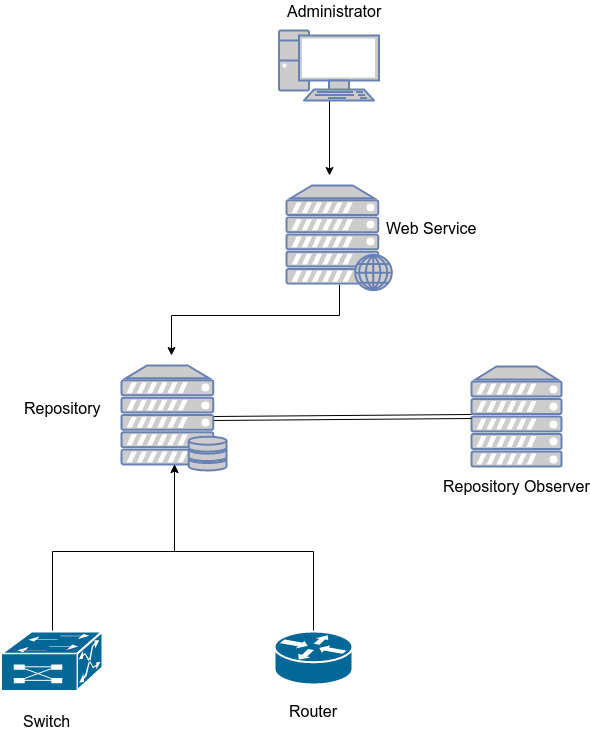
\includegraphics[width=8cm,height=10cm]{Images/C-3/Middleware.png}
                    \caption{Desain \textit{Middleware}}
                    \label{desain:middleware}
				\end{figure}
            \indent \textit{HTTP Rest API} dibangun menggunakan Flask yang sudah terintegrasi gitPython dan Python watchdog. Modul gitPython dan Python Watchdog digunakan untuk mengamati repositori perangkat jaringan.
            
        \subsubsection{Perancangan \textit{Repository Observer}}
            Pada sistem ini Middleware harus bisa mengamati repositori perangkat jaringan secara berkelanjutan dan melakukan update pada history commit pada repositori. Untuk melakukan hal tersebut modul watchdog di dalam middleware yang akan melihat setiap perubahan pada respositori perangkat jaringan. Modul watchdog berjalan sebagai thread yang menunggu perubahan kondisi di dalam repositori. Ketika thread mengidentifikasi ada perubahan di dalam repositori maka thread akan menjalankan perintah commit menggunakan modul gitPython yang terintegrasi dengan middleware.
            \begin{figure}[H]
            	\centering
            	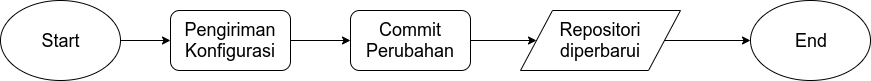
\includegraphics[width=10cm,height=1cm]{Images/C-3/AlurPengirimanFile.png}
            	\caption{Alur Pengiriman File}
            	\label{desain:pengiriman file}
            \end{figure}
	        \indent Repository Observer juga mengatur pembentukan cabang dari repositori penyimpanan konfigurasi perangkat jaringan. Alur pembuatan cabang dari repositori seperti pada gambar \ref{CreateBranch}.
	        \begin{figure}[H]
	        	\centering
	        	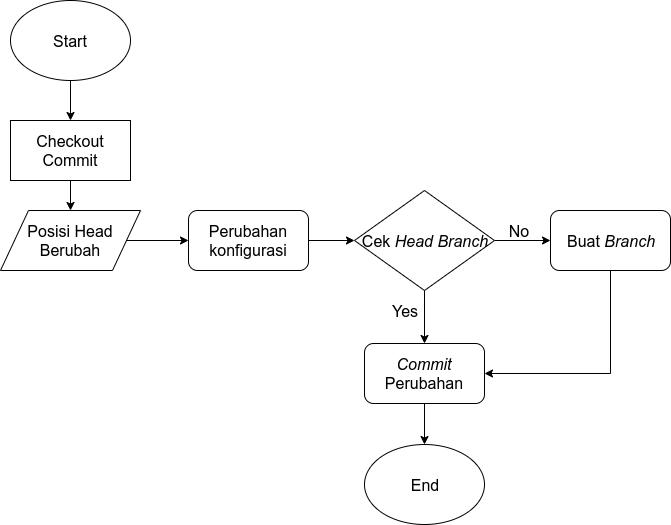
\includegraphics[width=\textwidth]{Images/C-3/CreateBranch.png}
	        	\caption{Alur Pembuatan Branch}
	        	\label{CreateBranch}
	        \end{figure}
        
        
        \subsubsection{Perancangan Web \textit{Service}}
        	Dalam sistem yang dibangun, web service digunakan untuk menerjemahkan permintaan dari adiministrator jaringan. Web service memiliki antarmuka dan rute dengan parameter nama repositori dan permintaan fitur yang diinginkan. Setiap rute akan diproses oleh \textit{Middleware} dan kemudian mengirimkan respon kepada administrator.
         	
        
       
            
        